\documentclass[a4paper]{book}
\usepackage{a4wide}
\usepackage{makeidx}
\usepackage{graphicx}
\usepackage{multicol}
\usepackage{float}
\usepackage{listings}
\usepackage{color}
\usepackage{textcomp}
\usepackage{alltt}
\usepackage{times}
\usepackage[utf8]{inputenc}
\usepackage{doxygen}
\lstset{language=C++,inputencoding=utf8,basicstyle=\footnotesize,breaklines=true,breakatwhitespace=true,tabsize=8,numbers=left }
\makeindex
\setcounter{tocdepth}{3}
\renewcommand{\footrulewidth}{0.4pt}
\begin{document}
\begin{titlepage}
\vspace*{7cm}
\begin{center}
{\Large Compressor }\\
\vspace*{1cm}
{\large Generated by Doxygen 1.6.3}\\
\vspace*{0.5cm}
{\small Mon May 30 22:44:43 2011}\\
\end{center}
\end{titlepage}
\clearemptydoublepage
\pagenumbering{roman}
\tableofcontents
\clearemptydoublepage
\pagenumbering{arabic}
\chapter{Class Index}
\section{Class Hierarchy}
This inheritance list is sorted roughly, but not completely, alphabetically:\begin{DoxyCompactList}
\item \contentsline{section}{caracter}{\pageref{structcaracter}}{}
\item \contentsline{section}{Codec}{\pageref{classCodec}}{}
\begin{DoxyCompactList}
\item \contentsline{section}{CodecHuffman}{\pageref{classCodecHuffman}}{}
\item \contentsline{section}{CodecLZW}{\pageref{classCodecLZW}}{}
\end{DoxyCompactList}
\item \contentsline{section}{No}{\pageref{classNo}}{}
\end{DoxyCompactList}

\chapter{Class Index}
\section{Class List}
Here are the classes, structs, unions and interfaces with brief descriptions:\begin{DoxyCompactList}
\item\contentsline{section}{{\bf caracter} }{\pageref{structcaracter}}{}
\item\contentsline{section}{{\bf Codec} }{\pageref{classCodec}}{}
\item\contentsline{section}{{\bf CodecHuffman} }{\pageref{classCodecHuffman}}{}
\item\contentsline{section}{{\bf CodecLZW} }{\pageref{classCodecLZW}}{}
\item\contentsline{section}{{\bf No} }{\pageref{classNo}}{}
\end{DoxyCompactList}

\chapter{Class Documentation}
\section{caracter Struct Reference}
\label{structcaracter}\index{caracter@{caracter}}
\subsection*{Public Attributes}
\begin{DoxyCompactItemize}
\item 
unsigned char {\bfseries c}\label{structcaracter_a5bda935cece7d3513d2c3787a749844f}

\item 
string {\bfseries representacao}\label{structcaracter_a6e730c7b52e446b727e5a400538bec7a}

\end{DoxyCompactItemize}


The documentation for this struct was generated from the following file:\begin{DoxyCompactItemize}
\item 
src/ArvoreBinaria.h\end{DoxyCompactItemize}

\section{Codec Class Reference}
\label{classCodec}\index{Codec@{Codec}}


{\ttfamily \#include $<$Codec.h$>$}

Inheritance diagram for Codec:\begin{figure}[H]
\begin{center}
\leavevmode
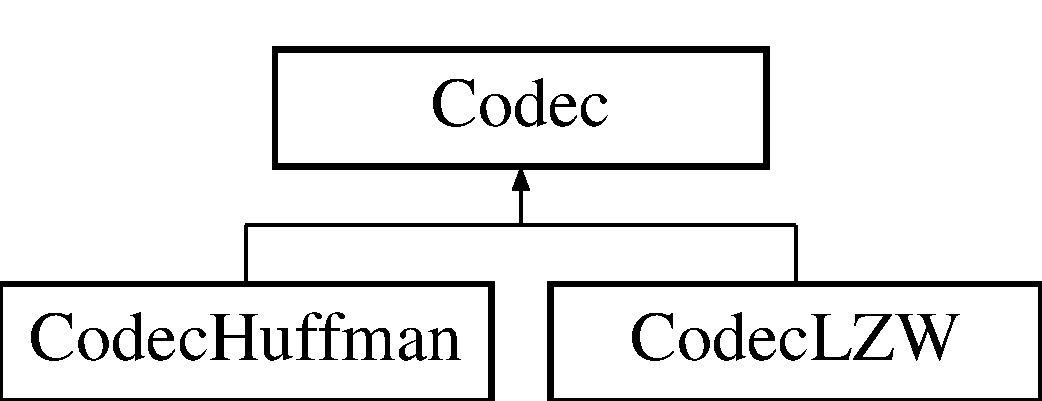
\includegraphics[height=2cm]{classCodec}
\end{center}
\end{figure}
\subsection*{Public Member Functions}
\begin{DoxyCompactItemize}
\item 
{\bf Codec} (string file)
\item 
virtual string {\bf decomprimir} ()=0
\end{DoxyCompactItemize}
\subsection*{Protected Attributes}
\begin{DoxyCompactItemize}
\item 
string {\bfseries filename}\label{classCodec_ad4cbcb9e265245e0ed0d3440e1913d6b}

\end{DoxyCompactItemize}


\subsection{Detailed Description}
Classe abstracta que representa um codec. 

\subsection{Constructor \& Destructor Documentation}
\index{Codec@{Codec}!Codec@{Codec}}
\index{Codec@{Codec}!Codec@{Codec}}
\subsubsection[{Codec}]{\setlength{\rightskip}{0pt plus 5cm}Codec::Codec (string {\em file})\hspace{0.3cm}{\ttfamily  [inline]}}\label{classCodec_a42a57ddd33236ac3e30decd6c673a4fb}
Constructor de um codec. Recebe o nome do ficheiro a carregar para comprimir ou descomprimir


\begin{DoxyParams}{Parameters}
\item[{\em file}]nome do ficheiro \end{DoxyParams}


\subsection{Member Function Documentation}
\index{Codec@{Codec}!decomprimir@{decomprimir}}
\index{decomprimir@{decomprimir}!Codec@{Codec}}
\subsubsection[{decomprimir}]{\setlength{\rightskip}{0pt plus 5cm}virtual string Codec::decomprimir ()\hspace{0.3cm}{\ttfamily  [pure virtual]}}\label{classCodec_a371347b9b3be1e237f92454244c43b38}
Decomprime o ficheiro

\begin{DoxyReturn}{Returns}
texto do ficheiro 
\end{DoxyReturn}


Implemented in {\bf CodecHuffman} \doxyref{}{p.}{classCodecHuffman_a5098f57bd6bc4df66b400e1ff4154443}, and {\bf CodecLZW} \doxyref{}{p.}{classCodecLZW_a645e1bd0b97bed0222c768318ee75bbc}.



The documentation for this class was generated from the following file:\begin{DoxyCompactItemize}
\item 
src/Codec.h\end{DoxyCompactItemize}

\section{CodecHuffman Class Reference}
\label{classCodecHuffman}\index{CodecHuffman@{CodecHuffman}}


{\ttfamily \#include $<$Codec.h$>$}

Inheritance diagram for CodecHuffman:\begin{figure}[H]
\begin{center}
\leavevmode
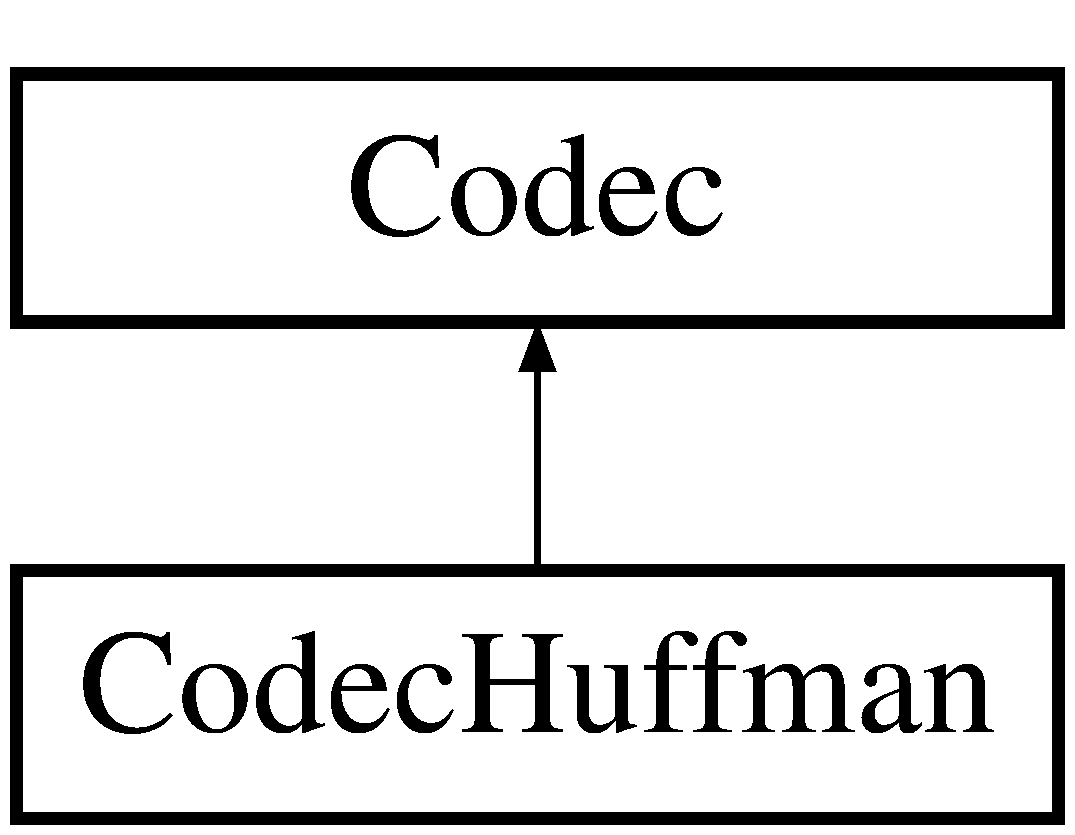
\includegraphics[height=2cm]{classCodecHuffman}
\end{center}
\end{figure}
\subsection*{Public Member Functions}
\begin{DoxyCompactItemize}
\item 
{\bfseries CodecHuffman} (string file)\label{classCodecHuffman_aa30983418c652a7a4a9002ec7d165ecb}

\item 
vector$<$ byte $>$ {\bfseries comprimir} ()\label{classCodecHuffman_a7c70008177329e96f5f1e9a1b546caa3}

\item 
string {\bf decomprimir} ()
\end{DoxyCompactItemize}


\subsection{Detailed Description}
\doxyref{Codec}{p.}{classCodec} que usa os codigos de Huffman 

\subsection{Member Function Documentation}
\index{CodecHuffman@{CodecHuffman}!decomprimir@{decomprimir}}
\index{decomprimir@{decomprimir}!CodecHuffman@{CodecHuffman}}
\subsubsection[{decomprimir}]{\setlength{\rightskip}{0pt plus 5cm}string CodecHuffman::decomprimir ()\hspace{0.3cm}{\ttfamily  [virtual]}}\label{classCodecHuffman_a5098f57bd6bc4df66b400e1ff4154443}
Decomprime o ficheiro

\begin{DoxyReturn}{Returns}
texto do ficheiro 
\end{DoxyReturn}


Implements {\bf Codec} \doxyref{}{p.}{classCodec_a371347b9b3be1e237f92454244c43b38}.



The documentation for this class was generated from the following files:\begin{DoxyCompactItemize}
\item 
src/Codec.h\item 
src/CodeHuffman.cpp\end{DoxyCompactItemize}

\section{CodecLZW Class Reference}
\label{classCodecLZW}\index{CodecLZW@{CodecLZW}}


{\ttfamily \#include $<$Codec.h$>$}

Inheritance diagram for CodecLZW:\begin{figure}[H]
\begin{center}
\leavevmode
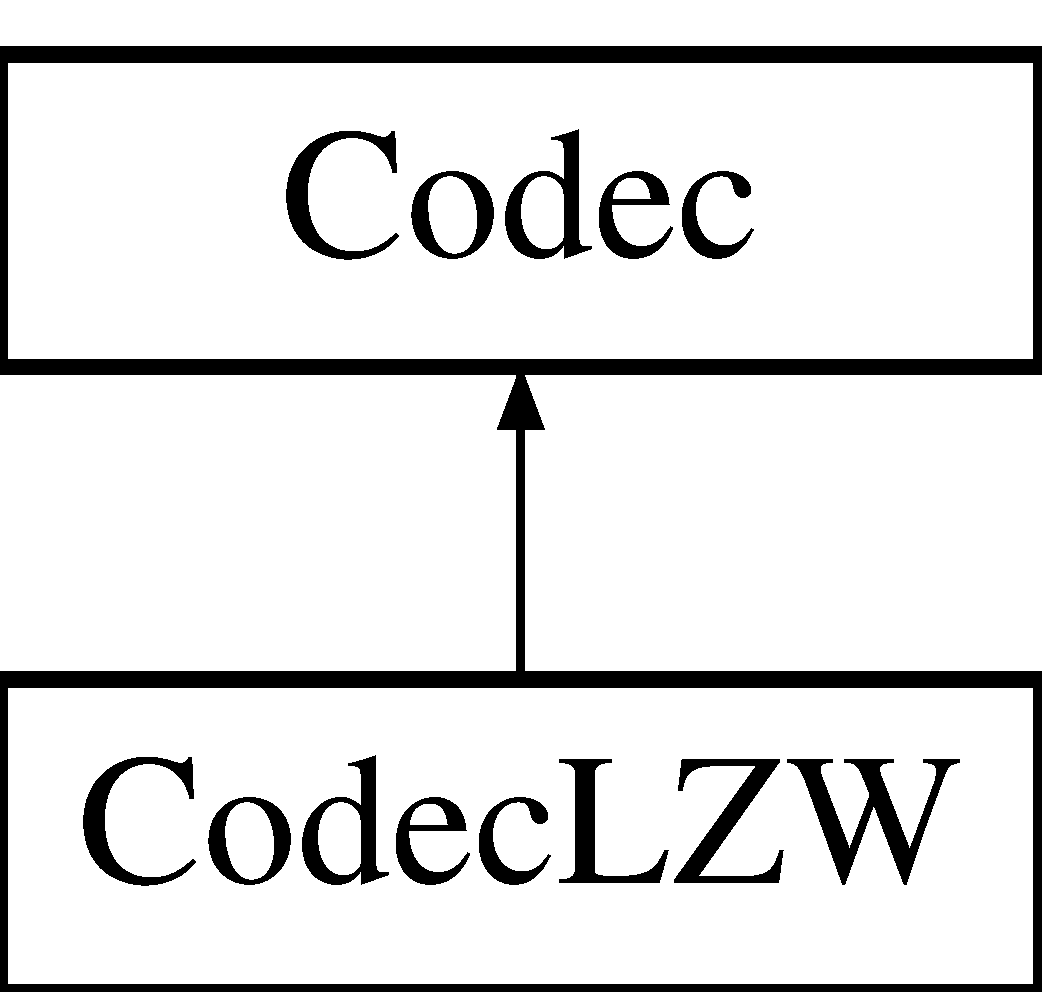
\includegraphics[height=2cm]{classCodecLZW}
\end{center}
\end{figure}
\subsection*{Public Member Functions}
\begin{DoxyCompactItemize}
\item 
{\bfseries CodecLZW} (string file)\label{classCodecLZW_a931dfb08d57e69d8b0d8e3fed626e8a0}

\item 
vector$<$ int $>$ {\bfseries comprimir} ()\label{classCodecLZW_afa8d9aa96427d373f8f8192044eb862f}

\item 
string {\bf decomprimir} ()
\item 
void {\bfseries setDicCompress} (map$<$ string, int $>$ d)\label{classCodecLZW_adef0bb2823fa2f9a098a25d34d812e52}

\item 
map$<$ string, int $>$ {\bfseries getDicCompress} ()\label{classCodecLZW_aa180fc37e4a838549660195f54ac1955}

\end{DoxyCompactItemize}
\subsection*{Protected Attributes}
\begin{DoxyCompactItemize}
\item 
int {\bfseries size}\label{classCodecLZW_a3caa21c252cb675da44f0615e5d05e90}

\item 
map$<$ string, int $>$ {\bfseries dictionaryCompress}\label{classCodecLZW_a2eb73d4b326fd77e89f425ed5017dc69}

\item 
map$<$ int, string $>$ {\bfseries dictionaryDecompress}\label{classCodecLZW_a6d36b72d8ab9a61a068cb3ddf8a47416}

\end{DoxyCompactItemize}


\subsection{Detailed Description}
\doxyref{Codec}{p.}{classCodec} que usa Lempel-\/Ziv-\/Welch 

\subsection{Member Function Documentation}
\index{CodecLZW@{CodecLZW}!decomprimir@{decomprimir}}
\index{decomprimir@{decomprimir}!CodecLZW@{CodecLZW}}
\subsubsection[{decomprimir}]{\setlength{\rightskip}{0pt plus 5cm}string CodecLZW::decomprimir ()\hspace{0.3cm}{\ttfamily  [virtual]}}\label{classCodecLZW_a645e1bd0b97bed0222c768318ee75bbc}
Decomprime o ficheiro

\begin{DoxyReturn}{Returns}
texto do ficheiro 
\end{DoxyReturn}


Implements {\bf Codec} \doxyref{}{p.}{classCodec_a371347b9b3be1e237f92454244c43b38}.



The documentation for this class was generated from the following files:\begin{DoxyCompactItemize}
\item 
src/Codec.h\item 
src/CodecLZW.cpp\end{DoxyCompactItemize}

\section{No Class Reference}
\label{classNo}\index{No@{No}}
\subsection*{Public Member Functions}
\begin{DoxyCompactItemize}
\item 
{\bfseries No} (unsigned char c, int p)\label{classNo_a052bb0ab26f8363ba7cd2c480374f63c}

\item 
void {\bfseries addNo} ({\bf No} $\ast$n)\label{classNo_a8bedf6aad116e54bb0fc22d1e044f9f1}

\item 
{\bf No} $\ast$ {\bfseries getEsquerda} ()\label{classNo_a4332d6147b190dd87e1782b98ed0ff4f}

\item 
{\bf No} $\ast$ {\bfseries getDireita} ()\label{classNo_a4a7550a43a59338edb4c7d7f2440fac9}

\item 
int {\bfseries getPeso} ()\label{classNo_a6c842040108547560c2c371a8b0c26bc}

\item 
unsigned char {\bfseries getChar} ()\label{classNo_a010acaa9f44b43f2c237cfd70b4fd80e}

\item 
bool {\bfseries isFolha} ()\label{classNo_abc1a6962dab9ec0ded8a11486cb309a9}

\end{DoxyCompactItemize}


The documentation for this class was generated from the following files:\begin{DoxyCompactItemize}
\item 
src/ArvoreBinaria.h\item 
src/ArvoreBinaria.cpp\end{DoxyCompactItemize}

\printindex
\end{document}
